\section{Zadanie 3}
\autor{Aleksander Wieczorek}
Jaka jest wartość oczekiwana i wariancja zmiennej X z poprzedniego zadania?
\subsection*{Rozwiązanie}
Załóżmy że w talii mamy tylko C czarnych nierozróżnialnych kart. Jeśli je ponumerujemy możemy wskazać r-tą z nich. Teraz zdefiniujmy indykator:
\[X_i=\begin{cases}
		1\text{ - jeśli i-ta karta będzie odkryta} \\
		0 \text{ - w p.p.}
	\end{cases}\]
fakt, że i-ta karta będzie odkryta jest równoważny z tym, że znajduje się przed r-tą czarną kartą w talii.\\
Możemy teraz rozważyć dla każdej i-tej karty gdzie może się znaleźć względem czarnych kart:
\vspace{5mm}
\begin{figure}[ht!]
	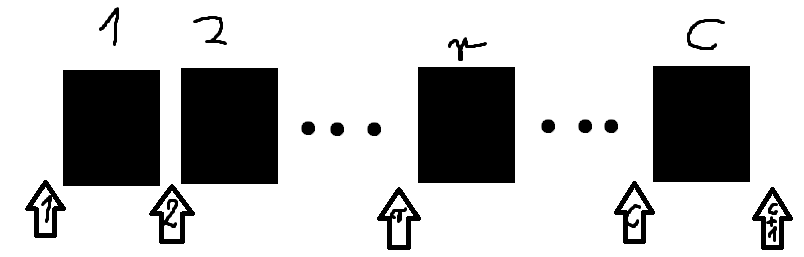
\includegraphics[width=\textwidth]{./tasks/03.png}
	\caption{Gdzie może trafić biała karta}
	\label{fig:placeholder}
\end{figure}
Z własności indykatorów i rysunku dostajemy:
\[E(X_i)=P(X_i=1)=\frac{r}{C+1}\]
A z liniowości mamy:
\[E(X)=E(\sum_{i=1}^B X_i)=\sum_{i=1}^BE(X_i) = B\frac{r}{C+1}\]
Teraz możemy policzyć wariancję.
\[Var(X)=E(X^2)-E(X)^2\]
\[E(X^2)=\sum_{i=1}^B E(X_i^2) + \sum_{i\ne j} E(X_iX_j)\]
Z własności indykatorów mamy \(E(X_i^2)=E(X_i)\), dla 2. części sumy:
\[E(X_iX_j)=P(X_i=1\cap X_j=1) =\frac{r}{C+1}\frac{r+1}{C+2}  \]
1. przekształcenie wynika z własności indykatorów, w 2. po wstawieniu poprawnie 1. karty pojawia się dodatkowy slot, który jest dobry.
Wracając:
\[E(X^2)=B\frac{r}{C+1} + B(B-1)\frac{r}{C+1}\frac{r+1}{C+2} \]
podstawiając do wariancji:
\[Var(X)=B\frac{r}{C+1} + B(B-1)\frac{r}{C+1}\frac{r+1}{C+2}  -  \left(B\frac{r}{C+1}\right)^2\]
\[=\frac{Br}{C+1}\left( 1 +\frac{(B-1)(r+1)}{C+2}-\frac{Br}{C+1}   \right)\]
\subsection*{Odpowiedź}
\[E(X)= \frac{Br}{C+1}\]
\[Var(X)=\frac{Br}{C+1}\left( 1 +\frac{(B-1)(r+1)}{C+2}-\frac{Br}{C+1}   \right)\]
